% ---------------------------------------------------------------
% Preamble
% ---------------------------------------------------------------
\documentclass[a4paper,11pt]{book}
% ---------------------------------------------------------------
% Includes arcticle-specific preamble configurations
% --------------------------------------------------------------------
% Packages
% --------------------------------------------------------------------
% Text, input, formatting, and language-related packages
\usepackage[T1]{fontenc}
\usepackage[utf8]{inputenc}
\usepackage[english]{babel}
\usepackage[protrusion=true,expansion=true,final]{microtype} 
\usepackage{lmodern}

% Margin and formatting specifications
\usepackage[margin=1in,a4paper,pdftex]{geometry}      
\usepackage[style=abnt,giveninits=true,block=space,noslsn,pretty,maxcitenames=2,maxbibnames=99]{biblatex}

% Math packages
\usepackage{amsmath,amsfonts,amsthm,amssymb,bm,mathdots,mathtools,bigints}

% TiKz packages
\usepackage{tikz, pgfplots, tikzsymbols, tikzducks}

% Graphic and color packages
\usepackage[export]{adjustbox}				% Environment to adjust LaTeX objects
\usepackage[skins]{tcolorbox}				% Coloured boxes for LaTeX objects
\usepackage{graphicx} 						% Enhanced support for graphics
\usepackage{color, xcolor}					% Driver-independent color extensions
\usepackage{wrapfig}						% Environment to wrap figures/tables
\usepackage{caption}                        % Tools for customizing the \caption{} command
\usepackage{subcaption}						% Environment to create subcaptions

% General utilities
\usepackage[nodayofweek]{datetime}			% Customize date commands
\usepackage[document]{ragged2e}				% Text-alignment (\centering, ...)
\usepackage[ruled, vlined]{algorithm2e}		% Pseudo-code environment
\usepackage{titlesec}                       % Customizable titles for chapters
\usepackage{fancyhdr}                       % Extensive control of headers/footnotes
\usepackage{titling}                        % Control title typesetting (and variables)
\usepackage{framed, mdframed}				% Framed and shaded environments
\usepackage{multicol,multirow}				% Multicolumn and Multirow environments
\usepackage{enumerate}						% More functionalities for {enumerate}
\usepackage{environ}						% Better interface for environments
\usepackage{listings}						% Coding environments
\usepackage{etoolbox,xstring}				% Environment hooks (\BeforeBegin...)
\usepackage{hyperref}                       % Color and helps using hyperlinks
\usepackage{tabularx}                       % Customizable {tabular} environments
\usepackage{tocloft}                        % Customizable table of contents pages
\usepackage{indentfirst}                    % Add identation to first paragraph on sects
\usepackage{parskip,setspace}               % Tools for changing skip, stretchs, etc
\usepackage{chngcntr}                       % Allows for contiguous figure numbering
\usepackage{makecell}                       % A \makecell{} comand for Table envs
\usepackage{lipsum}                         % Lorem ipsum generator

% --------------------------------------------------------------------
% Other Definitions
% --------------------------------------------------------------------
% Additional cool colors
\definecolor{stateColor}{RGB}{224,60,48}		% e03c30ff
\definecolor{inputColor}{RGB}{73,158,255}		% 
\definecolor{disturbanceColor}{RGB}{102,43,153} % 662b99ff
\definecolor{outputColor}{cmyk}{0.82,0,0.92,0}  % 21b20eff, RGB(33,178,14)
\definecolor{paramColor}{RGB}{224,148,48}

\definecolor{myYellow}{rgb}{1,0.65,0}
\definecolor{myRed}{rgb}{0.84, 0.18, 0.13}
\definecolor{myGreen}{rgb}{0, 0.53, 0.27}
\definecolor{myBlue}{rgb}{0, 0.34, 0.91}

\definecolor{plotBlue}{rgb}{0, 0.4470, 0.7410}
\definecolor{plotRed}{rgb}{0.6350, 0.0780, 0.1840}

\definecolor{UFCBlue}{RGB}{0, 83, 134}
\definecolor{UFCGreen}{RGB}{0, 146, 62}
\definecolor{UFCOrange}{RGB}{231, 120, 19}

\definecolor{glgRed}{RGB}{214,45,32}
\definecolor{glgGreen}{RGB}{0,135,68}
\definecolor{glgBlue}{RGB}{0,87,231}
\definecolor{glgOrange}{RGB}{255,167,0}

\definecolor{retroBrown}{RGB}{102,101,71}
\definecolor{retroRed}{RGB}{251,46,1}
\definecolor{retroGreen}{RGB}{111,203,159}
\definecolor{retroYellow}{RGB}{255,226,138}

\definecolor{pastelBlue}{RGB}{27,133,184}
\definecolor{pastelRed}{RGB}{174,90,65}
\definecolor{pastelGreen}{RGB}{85,158,131}
\definecolor{pastelBlack}{RGB}{90,82,85}

\definecolor{niceBlack}{RGB}{14,17,17}
\definecolor{niceBlue}{RGB}{14,104,206}

\definecolor{monokaiBG}{RGB}{39,40,34}
\definecolor{monokaiOrange}{RGB}{253,151,31}
\definecolor{monokaiGreen}{RGB}{166,226,46}
\definecolor{monokaiBlue}{RGB}{102,217,239}
\definecolor{monokaiPink}{RGB}{249,38,114}

% --------------------------------------------------------------------
% Packages Configurations
% --------------------------------------------------------------------
% (inputenc, fontenc): Set serif on math fonts
% \usefonttheme[onlymath]{serif} 
\renewcommand{\familydefault}{\rmdefault}

% (hypperlink)
\hypersetup{colorlinks=true, linkcolor=myBlue!60!black, urlcolor=plotBlue, anchorcolor=plotBlue, citecolor=myRed!60!black}

% (tikz): Imports some custom libraries and pgfplot settings
\usetikzlibrary{shapes, arrows, decorations.pathmorphing}
\usetikzlibrary{backgrounds, positioning, fit, calc}
\usetikzlibrary{bayesnet, graphs}

\pgfplotsset{compat=1.16} 

% (minted): Set Monokai as default color style
%\usemintedstyle{monokai}
\definecolor{bg}{HTML}{282828} % (Source: https://github.com/kevinsawicki/monokai) 

% (listings): Defines the code styling and formatting
\lstset{
    backgroundcolor=\color[RGB]{142,142,142},
    language=matlab, keywordstyle=\color[RGB]{102,217,239},
    basicstyle=\footnotesize \ttfamily,breaklines=true,
    escapeinside={\%*}{*)}
}

% (caption): Configure the caption fonts and alignments and extra labels
\DeclareCaptionJustification{captionjustify}{\justifying}
\captionsetup{font=small, labelfont=bf, justification=captionjustify, singlelinecheck=on}

\DeclareCaptionLabelFormat{andtable}{#1~#2  \&  \tablename~\thetable}
\DeclareCaptionLabelFormat{andfigure}{#1~#2  \&  \figurename~\thefigure}

% (datetime): Personalized date commands (apply them before a \today)
\newdateformat{datenum}{\twodigit{\THEDAY}/\twodigit{\THEMONTH}/\THEYEAR}
\newdateformat{datefull}{\twodigit{\THEDAY}{ }\monthname[\THEMONTH], \THEYEAR}
\newdateformat{datefullpt}{\twodigit{\THEDAY}{ de }\monthname[\THEMONTH] de \THEYEAR}
\newdateformat{dateday}{\twodigit{\THEDAY}}
\newdateformat{dateyear}{\THEYEAR}

% (amsthm): Define new environments/numbering from Theorem environments
\numberwithin{figure}{chapter}
\numberwithin{equation}{chapter}
\numberwithin{table}{chapter}

\newtheorem{theorem}{Theorem}[chapter]
\newtheorem{corollary}{Corollary}[theorem]
\newtheorem{lemma}[theorem]{Lemma}

\theoremstyle{definition}
\newtheorem{definition}{Definition}[chapter]
\newtheorem{example}{Example}[chapter]

% (tocloft): Customize the Table of Contents identation
\setlength{\cftsecindent}{0pt}          % Remove indent for \section
\setlength{\cftsubsecindent}{0pt}       % Remove indent for \subsection
\setlength{\cftsubsubsecindent}{0pt}    % Remove indent for \subsubsection
\setlength{\cftfigindent}{0pt}          % Remove indent for List of Figures
\setlength{\cfttabindent}{0pt}          % Remove indent for List of Tables

\setlength{\cftbeforetoctitleskip}{-3em}  % Remove space before title TOC
\setlength{\cftaftertoctitleskip}{0em}    % Remove space after title TOC
\setlength{\cftbeforeloftitleskip}{-3em}  % Remove space before title LOF
\setlength{\cftafterloftitleskip}{0em}    % Remove space after title LOF
\setlength{\cftbeforelottitleskip}{-3em}  % Remove space before title LOT
\setlength{\cftafterlottitleskip}{0em}    % Remove space after title LOT

\setlength{\cftbeforechapskip}{0.675em}   % Remove space before chapter in TOC
\setlength{\cftbeforepartskip}{1.25em}    % Remove space before part in TOC

% (etoolbox) Supress the page numbering on plain pages
\patchcmd{\part}{\thispagestyle{plain}}{\thispagestyle{empty}}{}{}

% (titlesec) Customize the spacing before chapter titles 
\titleformat{\chapter}[hang]{\normalfont\huge\bfseries}{\thechapter}{1em}{\huge}   
\titlespacing*{\chapter}{0pt}{-50pt}{20pt}

% (biblatex) Forgets about the last used author to avoid dashes in repeated cases
\makeatletter
    \AtEveryBibitem{\global\undef\bbx@lasthash}
\makeatother

\DeclareFieldFormat*{apacase}{\textbf{#1}}

% (fancyhdr) Customize header/footnote and page numbering position
\pagestyle{fancy}
\fancyhf{}
\fancyhead[RO, LE]{\thepage}
\renewcommand{\headrulewidth}{0pt} \renewcommand{\footrulewidth}{0pt} 

\fancypagestyle{plain}{% <==============================================
  \fancyhf{}
  \fancyhead[RO]{\thepage}
  \renewcommand{\headrulewidth}{0pt} \renewcommand{\footrulewidth}{0pt}%
}


% --------------------------------------------------------------------
% Tikz Macros
% --------------------------------------------------------------------
\tikzstyle{sectionBlock} = [draw, fill=blue!20, rectangle, minimum height=3em, minimum width=3em]
\tikzstyle{block} 	  = [draw, thick, fill=white, rectangle, minimum height=2.5em, minimum width=2.5em]
\tikzstyle{sum} 	  = [draw, fill=white, circle, node distance=1cm]
\tikzstyle{input}     = [coordinate]
\tikzstyle{output}    = [coordinate]



% --------------------------------------------------------------------
% Commands
% --------------------------------------------------------------------

% \maketitle ~> Generates the external cover (ABNT-style)
\makeatletter
\renewcommand\maketitle{%
    \thispagestyle{empty}
    \begin{center}
        
\includegraphics[width=2.5cm]{imgs/logo_ufc} \\%
        \textbf{\textsc{\institute}\\\textsc{\department}\\\textsc{\program}}\\
        \vskip3cm{\normalsize\MakeUppercase{\textbf{\@author}}} \\%
        \vskip3cm{\LARGE\textbf{\MakeUppercase{\@title}}\\}
        \vfill%%
        {\MakeUppercase{\bfseries\textsc{Fortaleza -- CE} \\%
        \dateyear\today}}
    \end{center}

    \clearpage
    \thispagestyle{empty}}
\makeatother

% \makeinternaltitle ~> Generates the external cover (ABNT-style)
\makeatletter
\newcommand\makeinternaltitle{%
    %-------------------------------------------- %
    % INTERNAL COVER
    \thispagestyle{empty}%
    \begin{center}
        \vspace{0cm}{\MakeUppercase{\@author}}\\%
        \vspace{3cm}{\Large\MakeUppercase{\@title}}\\%
    \end{center}\vspace{4cm}%
    \begin{flushright}
        \begin{minipage}{\textwidth-8cm}\justifying
        \noindent Dissertação de Mestrado apresentada ao {\program}, do {\department} da {\institute}, como requisito parcial para obtenção do Título de {\mstitle}. 
        \ifdefempty{\msfield}{}{Área de concentração: {\msfield}.}\\
        
        \noindent Orientador: \advisor.
        \ifdefempty{\coadvisor}{}{\\\noindent Co-Orientador: \coadvisor.}
        \end{minipage}
    \end{flushright}\vfill%
    \begin{center}
        {\MakeUppercase{\textsc{Fortaleza -- CE}\\\dateyear\today}}
    \end{center}
    \clearpage\thispagestyle{empty}$\ $%
    %------------------------------------------- %
    % APPROVAL PAGE
    \clearpage\thispagestyle{empty}%
    \begin{center}
        \vspace{0cm}{\MakeUppercase{\@author}}\\%
        \vspace{3cm}{\Large\MakeUppercase{\@title}}\\%
    \end{center}\vspace{2cm}%
    \begin{flushright}
        \begin{minipage}{\textwidth-8cm}\justifying
        \noindent Dissertação de Mestrado apresentada ao {\program}, do {\department} da {\institute}, como requisito parcial para obtenção do Título de {\mstitle}. 
        \ifdefempty{\msfield}{}{Área de concentração: {\msfield}.}\\
        \end{minipage}
    \end{flushright}\vfill%
    \noindent Aprovada em: \_\_\_/\_\_\_/\_\_\_\_\_\_.
    \vfill%
    \begin{center}
        \noindent BANCA EXAMINADORA
        \vfill
        \csign{\textbf{\advisor} (Orientador)\\
            % \advisordepartment\\
            \advisorinstitute}
        \ifdefempty{\coadvisor}{}{\vfill%
        \csign{\textbf{\coadvisor} (Coorientador)\\
            % \coadvisordepartment\\
            \coadvisorinstitute}}
        \foreach \i in {1,...,\boardsize} {\vfill%
            \csign{\textbf{\pgfmathparse{\boardmembers[\i-1][0]}\pgfmathresult}\\
            % \pgfmathparse{\boardmembers[\i-1][1]}\pgfmathresult\\
            \pgfmathparse{\boardmembers[\i-1][2]}\pgfmathresult}}
    \end{center}
    \clearpage\thispagestyle{empty}$\ $}%
\makeatother

% \cftfigpresnum ~> Adds the text "Figure" in the List of Figures
\renewcommand{\cftfigpresnum}{Figure }
\renewcommand{\cftfigaftersnum}{ -}
\addtolength{\cftfignumwidth}{3.1em} % extra space for \cftpresnum

% \cftfigpresnum ~> Adds the text "Table" in the List of Tables
\renewcommand{\cfttabpresnum}{Table }
\renewcommand{\cfttabaftersnum}{ -}
\addtolength{\cfttabnumwidth}{2.75em} % extra space for \cftpresnum

% \contentsname ~> Redefine the Table of Contents/Figs/Tables titles to be centered
\renewcommand{\cfttoctitlefont}{\hfill\bfseries\Large\MakeUppercase} 
\renewcommand{\cftaftertoctitle}{\hfill}
\renewcommand{\cftchapdotsep}{\cftdotsep}

\renewcommand{\cftloftitlefont}{\hfill\bfseries\Large\MakeUppercase} 
\renewcommand{\cftafterloftitle}{\hfill}

\renewcommand{\cftlottitlefont}{\hfill\bfseries\Large\MakeUppercase} 
\renewcommand{\cftafterlottitle}{\hfill}

% Creates a doubled-hline to be used in Tabular enviornments (already has skips)
\newcommand\hlineskips{\rule{0pt}{3ex}\rule[-1ex]{0pt}{0pt}}
\newcommand\doublehline{\hline\hline\hlineskips}

% \blankpage ~> Adds a blank page (keeping the page counter constant)
\newcommand\blankpage{%
    \null
    \thispagestyle{empty}%
    \addtocounter{page}{-1}%
    \newpage}

% \printtitle ~> Prints the article title (NBR style)
\makeatletter                       
\def\printtitle{
    {\centering \@title\par}}
\makeatother                                    

% \printauthor ~> Prints the authors (NBR style)
\makeatletter 
\def\printauthor{
    {\centering \large \@author}}               
\makeatother                            

% \fullcite ~> Redeclares this function to use maxbibnames instead of maxnames
\makeatletter
\DeclareCiteCommand{\fullcite}
  {\defcounter{maxnames}{\blx@maxbibnames}%
    \usebibmacro{prenote}}
  {\usedriver
     {\DeclareNameAlias{sortname}{default}}
     {\thefield{entrytype}}}
  {\multicitedelim}
  {\usebibmacro{postnote}}
\DeclareCiteCommand{\footfullcite}[\mkbibfootnote]
  {\defcounter{maxnames}{\blx@maxbibnames}%
    \usebibmacro{prenote}}
  {\usedriver
     {\DeclareNameAlias{sortname}{default}}
     {\thefield{entrytype}}}
  {\multicitedelim}
  {\usebibmacro{postnote}}
\makeatother

% \tran ~> A cooler transpose symbol 'T'
\newcommand*{\tran}{{\mkern-1.5mu\mathsf{T}}}

% \tend & \tenq ~> Cool tensor sub- and super-scripts (\tend and \tenq, respectively)
\newcommand{\tend}[1]{\hbox{\oalign{$\bm{#1}$\crcr\hidewidth$\scriptscriptstyle\bm{\sim}$\hidewidth}}}
\newcommand{\tenq}[1]{\hbox{\oalign{$\bm{#1}$\crcr\hidewidth$\scriptscriptstyle\bm{\sim}$\hidewidth}}}

% \argmax & \argmin ~> Argmax and Argmin math operators
\DeclareMathOperator*{\argmax}{arg\,max}
\DeclareMathOperator*{\argmin}{arg\,min}

\newlength{\signwidth}
\setlength{\signwidth}{8.5cm}
\newlength{\signthickness}
\setlength{\signthickness}{0.05pt}
\newlength{\signskip}
\setlength{\signskip}{1.25cm}

\newcommand{\signcenter}{\@ifstar{\sign}{\csign}}

\newcommand{\sign}[1]{%
  \parbox{\signwidth}{\vspace*{\signskip}\centering%
  \rule{\signwidth}{\signthickness}\\%
  \nopagebreak #1\par}%
}

\newcommand{\csign}[1]%
  {\begingroup\par\centering\sign{#1}\par\endgroup}

\def\PARstartLetter#1#2{\begingroup\def\par{\endgraf\endgroup\lineskiplimit=0pt}
    \setbox2=\hbox{\xspace#2\hspace{0.4em}}\newdimen\tmpht \tmpht \ht2
    \advance\tmpht by \baselineskip\font\hhuge=cmr10 at \tmpht
    \setbox1=\hbox{{\hhuge \uppercase{#1}}}
    \count7=\tmpht \count8=\ht1\divide\count8 by 1000 \divide\count7 by\count8
    \tmpht=.001\tmpht\multiply\tmpht by \count7\font\hhuge=cmr10 at \tmpht
    \setbox1=\hbox{{\hhuge \uppercase{#1}}} \noindent \hangindent1.05\wd1
    \hangafter=-2 {\hskip-\hangindent \lower1\ht1\hbox{\raise1.0\ht2\copy1}%
    \kern-0\wd1}\copy2\lineskiplimit=-1000pt}


% --------------------------------------------------------------------
% Environments
% --------------------------------------------------------------------

% Slightly bigger equation environment
\NewEnviron{myequation*}
	{%
	\begin{equation*}
	\scalebox{1.1}{$\BODY$}
	\end{equation*}
	}

% A colored boxed environment for Theorems
\newcounter{boxedtheorem}
\makeatletter
\newenvironment{boxedtheorem}[1]
    {\colorlet{shadecolor}{black!4!white} \begin{shaded}\vspace*{-0.2cm} \begin{theorem}{#1}}
    {\end{theorem} \end{shaded}}

% A colored boxed environment for Lemma
\newcounter{boxedlemma}
\makeatletter
\newenvironment{boxedlemma}[1]
    {\colorlet{shadecolor}{black!4!white} \begin{shaded}\vspace*{-0.2cm} \begin{lemma}{#1}}
    {\end{lemma} \end{shaded}}

% A colored boxed environment for Definitions
\newcounter{boxeddefinition}
\makeatletter
\newenvironment{boxeddefinition}[1]
    {\colorlet{shadecolor}{black!4!white} \begin{shaded}\vspace*{-0.2cm} \begin{definition}{#1}}
    {\end{definition} \end{shaded}}

% A colored boxed environment for Examples
\newcounter{boxedexample}
\makeatletter
\newenvironment{boxedexample}[1]
    {\colorlet{shadecolor}{black!4!white} \begin{shaded}\vspace*{-0.2cm} \begin{example}{#1}}
    {\end{example} \end{shaded}}

% \makeatletter
% \newenvironment{proof}
%     {%
%     {\bf Proof.}%
%     }%
%     {%
%     \hfill$\blacksquare$
%     }%

\addbibresource{MscThesis_Aluno123456.bib}   % <~ Bibliography resources

% == Uncomment/change to toggle ABNT formatting ==
% \geometry{reset, inner=3cm, top=3cm, bottom=2cm, outer=2cm, a4paper, pdftex}                       

\titlespacing*{\chapter}{0pt}{-50pt}{0.5em}
\titlespacing*{\section}{0pt}{1em}{0.5em}
% == ==

\def\abntindent{0cm}  % <~ Change to 1.5cm for ABNT formatting
\def\abntstretch{1}   % <~ Change to 1.6 for ABNT formatting

% ---------------------------------------------------------------
% Metadata
% ---------------------------------------------------------------
% Title, authorship and affiliations
\title{Título título título}

\author{Aluno Aluno da Silva}
\def\institute{Universidade Federal do Ceará}
\def\department{Departamento de Engenharia de Teleinformática}

% Program name, title bestowed and research field
\def\program{Programa de Pós-graduação em Engenharia de Teleinformática}
\def\mstitle{Mestre em Engenharia de Teleinformática}
\def\msfield{Reconhecimento de Padrões e Sistemas Dinâmicos}

% Advisor and Co-Advisors (plus affiliations)
\def\advisor{Prof. Dr. Fulano Fulano}
\def\advisorinstitute{{\institute} (UFC)}
\def\advisordepartment{\department}

\def\coadvisor{Profa. Dra. Fulana Fulana}
\def\coadvisorinstitute{{\institute} (UFC)}
\def\coadvisordepartment{\department}

% Size and members of the defense board (and affiliations)
\def\boardsize{2}
\def\boardmembers{{{"Prof. Dr. XXXX", "Departamento de Coisas",  "Universidade ABC (UA)"}, 
                   {"Prof. Dr. YYYY", "Departamento de Negócio", "Universidade DEF (UD)"}}}


% ---------------------------------------------------------------
% Begin document
% ---------------------------------------------------------------
\begin{document}

% ==============================================================
% EXTERNAL COVER AND FRONT MATTER
% ==============================================================
\maketitle
%-----------------------------------------------------------------------------------------%
%----------------------------------INTERNAL COVER-----------------------------------------%
%-----------------------------------------------------------------------------------------%
\frontmatter
\makeinternaltitle

%-----------------------------------------------------------------------------------------%
%------------------------------------ DEDICATÓRIA ----------------------------------------%
%-----------------------------------------------------------------------------------------%
\clearpage\thispagestyle{empty}\null\vfill%

\begin{flushright}
    Dedico este trabalho aos [...].
\end{flushright}

\clearpage\thispagestyle{empty}$\ $% <~ Página vazia

%-----------------------------------------------------------------------------------------%
%----------------------------------- AGRADECIMENTOS --------------------------------------%
%-----------------------------------------------------------------------------------------%
\clearpage\thispagestyle{empty} \justifying

\begin{center} \bfseries \Large
    AGRADECIMENTOS
\end{center}
\vspace{1em}

\noindent Aos meus pais, [...]

\vspace{1em}

\noindent Aos meus orientadores, [...]

\vspace{1em}

\noindent Aos meus amigos [...]

\vspace{1em}

\noindent O presente trabalho foi realizado com apoio da Coordenação de Aperfeiçoamento de Pessoal de Nível Superior Brasil (CAPES) - Código de Financiamento 001.


%-----------------------------------------------------------------------------------------%
%------------------------------------- EPÍSTROFE -----------------------------------------%
%-----------------------------------------------------------------------------------------%
\clearpage\thispagestyle{empty}\null\vfill%

\begin{flushright}
    {\large \textit{``Citação.''}}\\ {\small Alguém (19\_\_)}
\end{flushright}

\clearpage\thispagestyle{empty}% <~ Página vazia

%-----------------------------------------------------------------------------------------%
%-------------------------------------- RESUMO -------------------------------------------%
%-----------------------------------------------------------------------------------------%
\clearpage\thispagestyle{empty} \justifying

\begin{center} \bfseries \Large
    RESUMO
\end{center}
\vspace{1em}

\PARstartLetter{O}{resumo} bla balb bla balba bal blabba ba bla blab balba lba alsdk maslkdma lskmdalsk dmsalkdm alskdm alkdmalsk md laskdmalskdm 

\lipsum[1-3]

\vskip0.3cm\noindent 
\textbf{Palavras-chave}: Chave 1, Chave 2, Chave 3. 

\clearpage\thispagestyle{empty}$\ $% <~ Página vazia

%-----------------------------------------------------------------------------------------%
%------------------------------------- ABSTRACT ------------------------------------------%
%-----------------------------------------------------------------------------------------%
\clearpage\thispagestyle{empty} \justifying

\begin{center} \bfseries \Large
    ABSTRACT
\end{center}
\vspace{1em}

\PARstartLetter{T}{he} abstract laksmfl askmfdl aksmflask dflaskmdfl skmfalsmfaosmf wmf mflms flsmf owme flskdmfa wemf lakdmfaoiemfa sldkfmowefms adkfm sl mskf masldkfm saldf masldkf masldkf masodfm akwemf sldfkmaoemfawlfkms dofmaw efmd lskfm owemif sldkmf s

\lipsum[1-3]

\vskip.3cm\noindent
\textbf{Keywords}: Key 1, Key 2, Key 3.

\clearpage\thispagestyle{empty}$\ $% <~ Página vazia

%-----------------------------------------------------------------------------------------%
%--------------------------------------FIGURAS--------------------------------------------%
%-----------------------------------------------------------------------------------------%
\clearpage\thispagestyle{empty}   
\listoffigures%

\addtocontents{toc}{\protect\thispagestyle{empty}}
\pagenumbering{gobble}
\clearpage\thispagestyle{empty}$\ $% <~ Página vazia

%-----------------------------------------------------------------------------------------%
%--------------------------------------TABELAS--------------------------------------------%
%-----------------------------------------------------------------------------------------%
\clearpage\thispagestyle{empty}   
\listoftables%

\addtocontents{toc}{\protect\thispagestyle{empty}}
\pagenumbering{gobble}
\clearpage\thispagestyle{empty}$\ $% <~ Página vazia

%-----------------------------------------------------------------------------------------%
%--------------------------------------SUMMARY--------------------------------------------%
%-----------------------------------------------------------------------------------------%
\clearpage
\setcounter{secnumdepth}{2}\setcounter{tocdepth}{1}
\tableofcontents%

\addtocontents{toc}{\protect\thispagestyle{empty}}
\pagenumbering{gobble} % <~ Edit this for Dedicatórias, Resumos, ...

% ==============================================================
% 1 - Introduction
\setstretch{\abntstretch}\setlength{\parindent}{\abntindent}%\setlength{\parskip}{0pt}

\clearpage\mainmatter\setcounter{page}{1}
% \part{Introduction} \label{part: Introduction}
% ==============================================================
% 1 - Introduction
% ==============================================================
\chapter{Introduction} \label{sec: Introduction}

\lipsum[1-2][4-8]

\section{Related publications} \label{sec: Introduction_Related_Publications}

During the development of this work, the following scientific contributions have been published:

\begin{itemize}
    \item [...]
\end{itemize}

\section{Thesis organization} \label{sec: Introduction_Thesis_Organization}

This document is organized into four parts, each comprised of a number of sections. 
\begin{enumerate}[I.]
    \item Chapter \ref{sec: Introduction} ... 
    %
    \item Chapter \ref{sec: Preliminaries} ... 
    %
    \item Chapter \ref{sec: Results} ... 
    %
    \item Chapter \ref{sec: Conclusion} ... 
\end{enumerate}

Furthermore, Appendix \ref{sec: Appendix} presents ... 


% ==============================================================
% 2 - Technical Background
% \part{Theoretical Preliminaries} \label{part: Theoretical_Background}
% ==============================================================
% 2 - Preliminaries
% ==============================================================
\chapter{Preliminaries} \label{sec: Preliminaries}

\lipsum[1-3]

\begin{figure}[htb!] \centering
    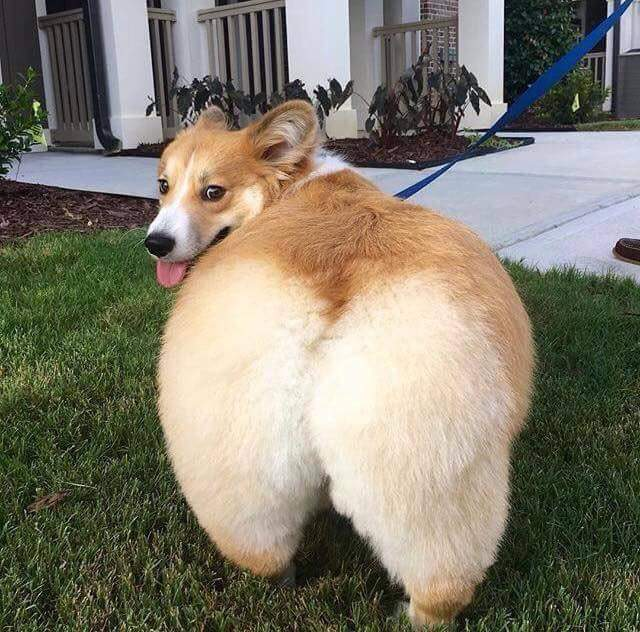
\includegraphics[width=0.6\textwidth]{imgs/dog.jpg}

    \caption{A dog, the inverse of a god.}
    \label{fig: Corgi}
\end{figure}

\lipsum[4-5]
\begin{align*}
    \dot{x}(t) &= A(t) x(t) + B(t) u(t) \\
          y(t) &= C(t) x(t) + D(t) u(t)
\end{align*}

\lipsum[6-8]

% ==============================================================
% 4 - Dynamical Properties of ASPs
% \part{Results and Discussions} \label{part: Results}
% ==============================================================
% 3 - Results and Discussion
% ==============================================================
\chapter{Results and Discussion} \label{sec: Results}

\lipsum[1-4]

\begin{table}[htb!] \centering
    \caption{Some numbers and some labels.}

    \begin{tabular}{l | c c c | l}
        Symbol   &   A1 &   A2 &   A3 & Units \\
        \doublehline
        $\alpha$ & 10.0 & 11.1 & 12.5 & m$^2$ \\ 
        $\beta$  & 31.2 & 21.2 & 82.1 & m$^2$ \\ 
        $\gamma$ & 64.5 & 14.1 & 22.5 & m$^2$
    \end{tabular} \vskip1em

    Source: Prepared by the author.
    \label{tab: Table_1}
\end{table}

\lipsum[3-4]
\begin{align*}
    x(t) = \Phi(t)x(0) + \int_{0}^{t} \Phi(t-\tau) B u(t) d\tau
\end{align*}

\lipsum[5-7]

% ==============================================================
% 5 - Conclusion
% \part{Conclusion} \label{part: Conclusion}
% ==============================================================
% 4 - Concluding Remarks
% ==============================================================
\chapter{Concluding remarks} \label{sec: Conclusion}

This work has presented [...]. The results show that:
\begin{itemize}
    \item ...
    \item ...
    \item ...
\end{itemize}


% ==============================================================
% Bibliography
% ==============================================================
\clearpage
\addcontentsline{toc}{chapter}{References}

\begin{center}\bfseries\Large
    REFERENCES
\end{center}
\vskip1em

{\justifying\setlength{\bibitemsep}{0.5em}\setstretch{1}
% \printbibliography[heading=none]}  % <------------------

% ==============================================================
% X - Apendices
% ==============================================================
\clearpage\appendix
% \part*{Appendix} \label{part: Appendix}
% ==============================================================
% Chapter: Appendix
% ==============================================================
\addcontentsline{toc}{chapter}{\hspace*{2.5em}Appendix A}
\chapter*{Appendix A} \label{sec: Appendix}
% ==============================================================

\lipsum[1-2]

\begin{boxedlemma}{\cite{Hautus1970}.} \label{def: Lemma_1}
	The following statements are all equivalent: 
	\begin{subequations} \begin{align}
		\text{\emph{ I}. }& \text{The pair $(A, C)$ is observable} \\
		\text{\emph{ II}. }&\texttt{rank}(\begin{bmatrix} \lambda I - A^{\tran}  & C^{\tran} \end{bmatrix}^{\tran} ) = N_x,  \text{ } \forall \lambda \in \mathbb{C}; \\
		\text{\emph{ III}. }&\texttt{rank}(\begin{bmatrix} \lambda_i I - A^{\tran}  &  C^{\tran} \end{bmatrix}^{\tran}) = N_x, \text{ } \forall \lambda_i \in \sigma(A) \subset \mathbb{C}.
	\end{align}	\end{subequations}
\end{boxedlemma}

\begin{proof}
	Left to the interested reader.
\end{proof}

\lipsum[1][1-6]

% ==============================================================
% End document
% ==============================================================
\end{document}